% Options for packages loaded elsewhere
\PassOptionsToPackage{unicode}{hyperref}
\PassOptionsToPackage{hyphens}{url}
\PassOptionsToPackage{dvipsnames,svgnames,x11names}{xcolor}
%
\documentclass[
  letterpaper,
  DIV=11,
  numbers=noendperiod]{scrartcl}

\usepackage{amsmath,amssymb}
\usepackage{iftex}
\ifPDFTeX
  \usepackage[T1]{fontenc}
  \usepackage[utf8]{inputenc}
  \usepackage{textcomp} % provide euro and other symbols
\else % if luatex or xetex
  \usepackage{unicode-math}
  \defaultfontfeatures{Scale=MatchLowercase}
  \defaultfontfeatures[\rmfamily]{Ligatures=TeX,Scale=1}
\fi
\usepackage{lmodern}
\ifPDFTeX\else  
    % xetex/luatex font selection
\fi
% Use upquote if available, for straight quotes in verbatim environments
\IfFileExists{upquote.sty}{\usepackage{upquote}}{}
\IfFileExists{microtype.sty}{% use microtype if available
  \usepackage[]{microtype}
  \UseMicrotypeSet[protrusion]{basicmath} % disable protrusion for tt fonts
}{}
\makeatletter
\@ifundefined{KOMAClassName}{% if non-KOMA class
  \IfFileExists{parskip.sty}{%
    \usepackage{parskip}
  }{% else
    \setlength{\parindent}{0pt}
    \setlength{\parskip}{6pt plus 2pt minus 1pt}}
}{% if KOMA class
  \KOMAoptions{parskip=half}}
\makeatother
\usepackage{xcolor}
\setlength{\emergencystretch}{3em} % prevent overfull lines
\setcounter{secnumdepth}{-\maxdimen} % remove section numbering
% Make \paragraph and \subparagraph free-standing
\ifx\paragraph\undefined\else
  \let\oldparagraph\paragraph
  \renewcommand{\paragraph}[1]{\oldparagraph{#1}\mbox{}}
\fi
\ifx\subparagraph\undefined\else
  \let\oldsubparagraph\subparagraph
  \renewcommand{\subparagraph}[1]{\oldsubparagraph{#1}\mbox{}}
\fi


\providecommand{\tightlist}{%
  \setlength{\itemsep}{0pt}\setlength{\parskip}{0pt}}\usepackage{longtable,booktabs,array}
\usepackage{calc} % for calculating minipage widths
% Correct order of tables after \paragraph or \subparagraph
\usepackage{etoolbox}
\makeatletter
\patchcmd\longtable{\par}{\if@noskipsec\mbox{}\fi\par}{}{}
\makeatother
% Allow footnotes in longtable head/foot
\IfFileExists{footnotehyper.sty}{\usepackage{footnotehyper}}{\usepackage{footnote}}
\makesavenoteenv{longtable}
\usepackage{graphicx}
\makeatletter
\def\maxwidth{\ifdim\Gin@nat@width>\linewidth\linewidth\else\Gin@nat@width\fi}
\def\maxheight{\ifdim\Gin@nat@height>\textheight\textheight\else\Gin@nat@height\fi}
\makeatother
% Scale images if necessary, so that they will not overflow the page
% margins by default, and it is still possible to overwrite the defaults
% using explicit options in \includegraphics[width, height, ...]{}
\setkeys{Gin}{width=\maxwidth,height=\maxheight,keepaspectratio}
% Set default figure placement to htbp
\makeatletter
\def\fps@figure{htbp}
\makeatother

\KOMAoption{captions}{tableheading}
\usepackage{fontspec}
\setmainfont{Times New Roman}
\usepackage{setspace}
\setstretch{1.25}
\fontsize{9pt}{12pt}\selectfont
\makeatletter
\makeatother
\makeatletter
\makeatother
\makeatletter
\@ifpackageloaded{caption}{}{\usepackage{caption}}
\AtBeginDocument{%
\ifdefined\contentsname
  \renewcommand*\contentsname{Table of contents}
\else
  \newcommand\contentsname{Table of contents}
\fi
\ifdefined\listfigurename
  \renewcommand*\listfigurename{List of Figures}
\else
  \newcommand\listfigurename{List of Figures}
\fi
\ifdefined\listtablename
  \renewcommand*\listtablename{List of Tables}
\else
  \newcommand\listtablename{List of Tables}
\fi
\ifdefined\figurename
  \renewcommand*\figurename{Figure}
\else
  \newcommand\figurename{Figure}
\fi
\ifdefined\tablename
  \renewcommand*\tablename{Table}
\else
  \newcommand\tablename{Table}
\fi
}
\@ifpackageloaded{float}{}{\usepackage{float}}
\floatstyle{ruled}
\@ifundefined{c@chapter}{\newfloat{codelisting}{h}{lop}}{\newfloat{codelisting}{h}{lop}[chapter]}
\floatname{codelisting}{Listing}
\newcommand*\listoflistings{\listof{codelisting}{List of Listings}}
\makeatother
\makeatletter
\@ifpackageloaded{caption}{}{\usepackage{caption}}
\@ifpackageloaded{subcaption}{}{\usepackage{subcaption}}
\makeatother
\makeatletter
\@ifpackageloaded{tcolorbox}{}{\usepackage[skins,breakable]{tcolorbox}}
\makeatother
\makeatletter
\@ifundefined{shadecolor}{\definecolor{shadecolor}{rgb}{.97, .97, .97}}
\makeatother
\makeatletter
\makeatother
\makeatletter
\makeatother
\ifLuaTeX
  \usepackage{selnolig}  % disable illegal ligatures
\fi
\IfFileExists{bookmark.sty}{\usepackage{bookmark}}{\usepackage{hyperref}}
\IfFileExists{xurl.sty}{\usepackage{xurl}}{} % add URL line breaks if available
\urlstyle{same} % disable monospaced font for URLs
\hypersetup{
  pdftitle={Walmart weekly sales mid-term project},
  pdfauthor={Yingmai Chen},
  colorlinks=true,
  linkcolor={blue},
  filecolor={Maroon},
  citecolor={Blue},
  urlcolor={Blue},
  pdfcreator={LaTeX via pandoc}}

\title{Walmart weekly sales mid-term project}
\author{Yingmai Chen}
\date{}

\begin{document}
\maketitle
\ifdefined\Shaded\renewenvironment{Shaded}{\begin{tcolorbox}[interior hidden, breakable, enhanced, borderline west={3pt}{0pt}{shadecolor}, sharp corners, frame hidden, boxrule=0pt]}{\end{tcolorbox}}\fi

\hypertarget{i.abstract}{%
\section{I.Abstract}\label{i.abstract}}

The project aims to find the relationship between weekly sales of
walmart with other variables,and also want to find which variable is
more correlated with weekly sales,and the project will include six
parts:``Abstract'',``Introduction'',``method'',``results'',``discussion'',``appendix''.
The first two parts are the descriptions of this project,and the method
part would have two parts:EDA(Exploratory Data Analysis),and model.The
results would be the comparison and illustration of the model.Discussion
part would discuss some future questions about my project,appendix would
include some poorly visualized graphs.

\hypertarget{ii.introduction}{%
\section{II.Introduction}\label{ii.introduction}}

In this study, we leveraged a dataset from Kaggle to identify and
quantify various factors impacting weekly sales. The dataset includes
key variables such as holidays, oil prices, temperature, unemployment
rates, and the Consumer Price Index (CPI), we utilized regression
analysis to assess the relative impact of these variables on sales
volumes.Through this study, we hope to offer a more comprehensive and
accurate sales forecasting model, helping businesses better understand
market dynamics and make more effective business decisions.

\hypertarget{iii.method}{%
\section{III.Method}\label{iii.method}}

I check the summary of the data first and see there don't have NA's in
the data,so we don't need to deal with the missing value of data.

\hypertarget{eda}{%
\subsection{EDA}\label{eda}}

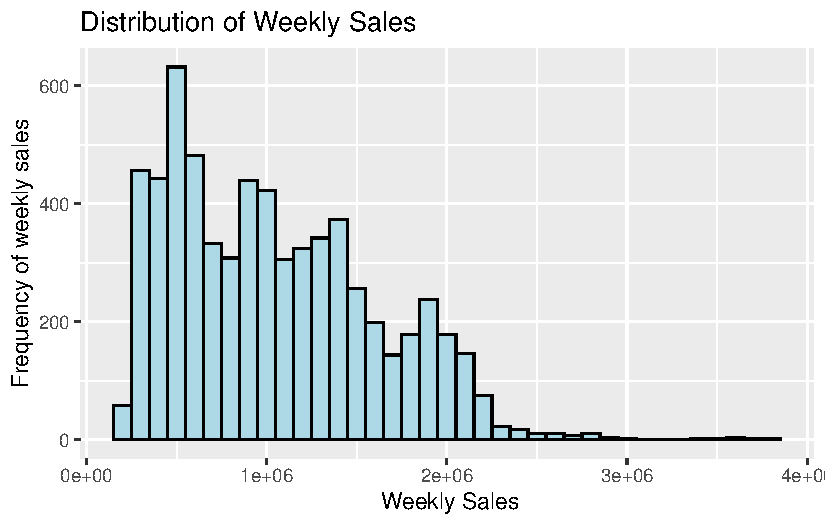
\includegraphics{678final_files/figure-pdf/unnamed-chunk-4-1.pdf}

From this plot,we can see that there are fewer weeks with very high
sales compared to weeks with low sales.This is typical for sales data
where a small number of periods (like holiday seasons) might have
exceptionally high sales.

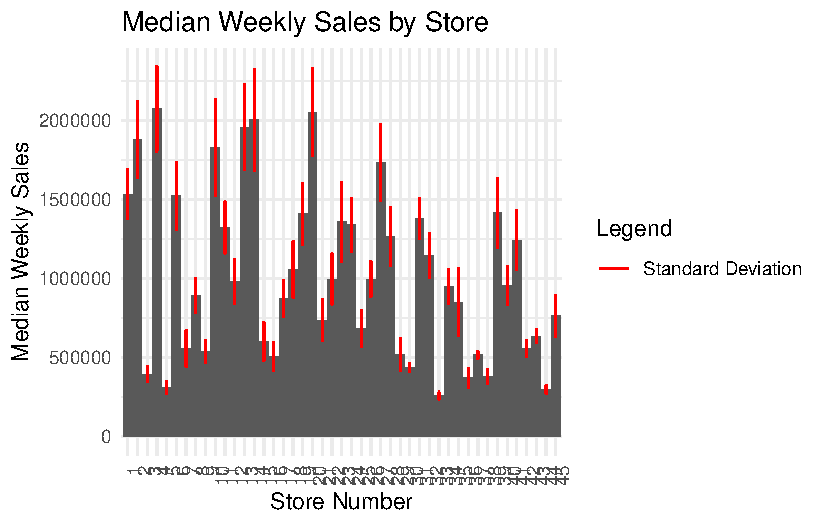
\includegraphics{678final_files/figure-pdf/unnamed-chunk-5-1.pdf}

From this plot,we can see there exist obvious differences between each
store,some has higher median of weekly sales, and some would have bigger
error bar which means sales are more volatile.this suggests that we
should trying multilevel model in the model part.

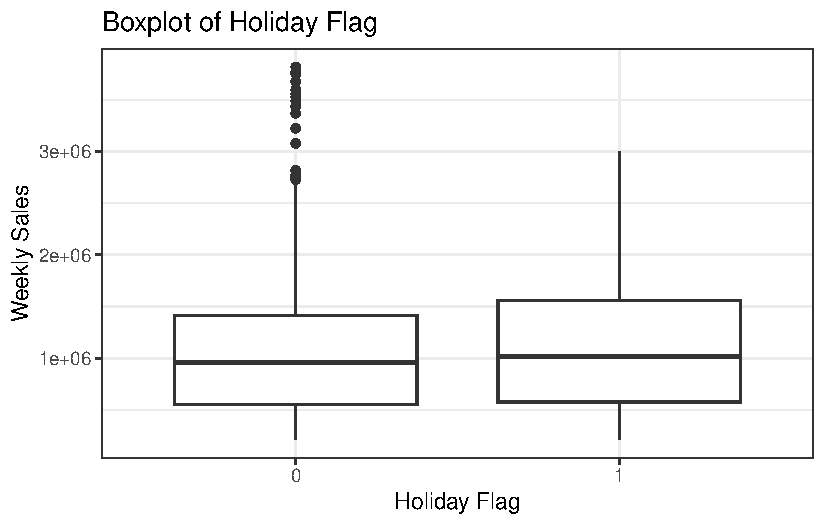
\includegraphics{678final_files/figure-pdf/unnamed-chunk-6-1.pdf}

From this plot,we can see the median of holiday weekly sales is a little
bit higher than non-holiday weekly sale, and the numbers of outliers in
non-holiday weekly sales are more than holiday-weekly sales,based on
this,I think there would have some relationships between holidays and
weekly sales.

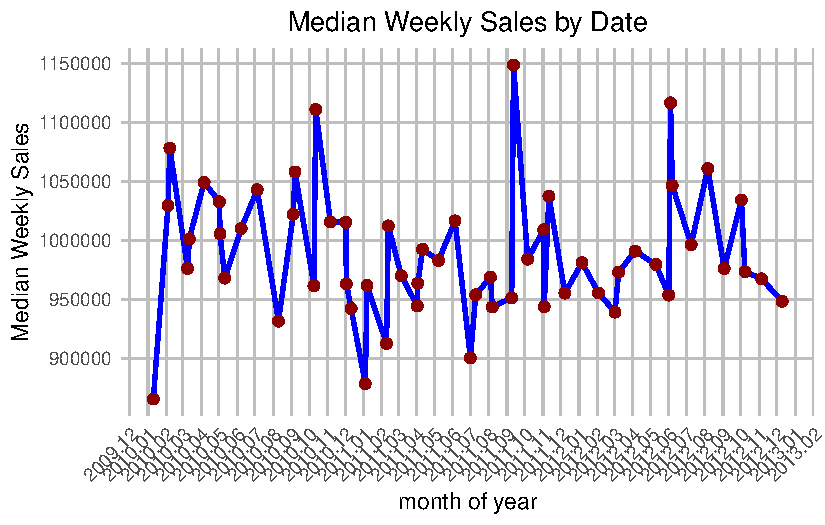
\includegraphics{678final_files/figure-pdf/unnamed-chunk-7-1.pdf}

From this plot,we can see that there is a recurring trend of lower sales
at the beginning of each year. This dip in sales could be attributed to
post-holiday season effects, where consumer spending typically drops
following the end-of-year holidays,which means the date would have
impact on weekly sales.

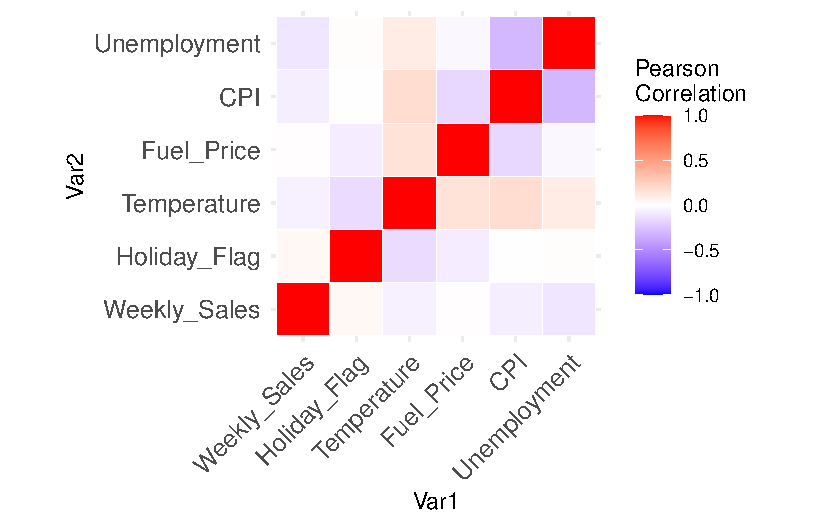
\includegraphics{678final_files/figure-pdf/unnamed-chunk-8-1.pdf}

As we can see, from this plot,It is not obvious that these variables are
correlated to weekly sales.

\hypertarget{model}{%
\subsection{model}\label{model}}

Because we can not easily draw a conclusion by doing EDA,so the next
step for us shoud be modeling,

\hypertarget{null-model}{%
\subsubsection{Null model}\label{null-model}}

\hypertarget{complete-pooling-model}{%
\subsubsection{complete pooling model}\label{complete-pooling-model}}

\hypertarget{no-pooling-model}{%
\subsubsection{No pooling model}\label{no-pooling-model}}

\hypertarget{generalized-linear-model}{%
\subsubsection{generalized linear
Model}\label{generalized-linear-model}}

\hypertarget{iv.result}{%
\section{IV.result}\label{iv.result}}

\hypertarget{v.discussion}{%
\section{V.discussion}\label{v.discussion}}

\hypertarget{vi.appendix}{%
\section{VI.appendix}\label{vi.appendix}}

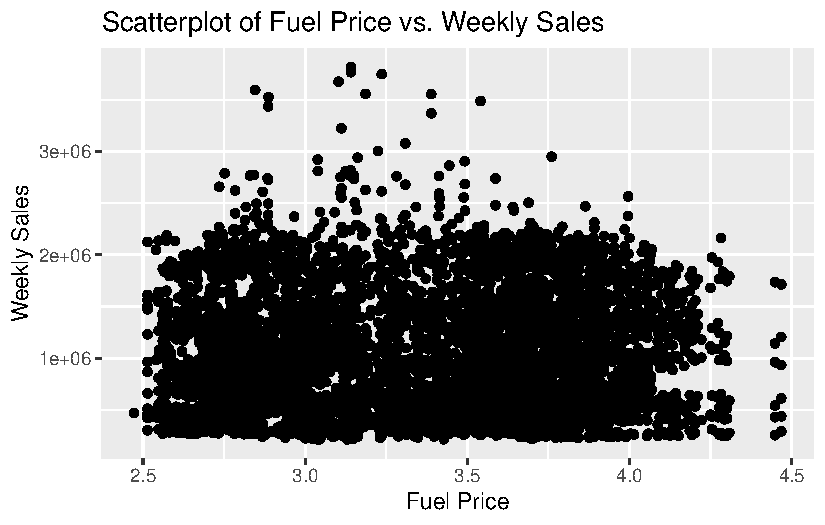
\includegraphics{678final_files/figure-pdf/unnamed-chunk-13-1.pdf}

From this plot, we can hardly see if there exist relationships between
CPI and weekly sales.

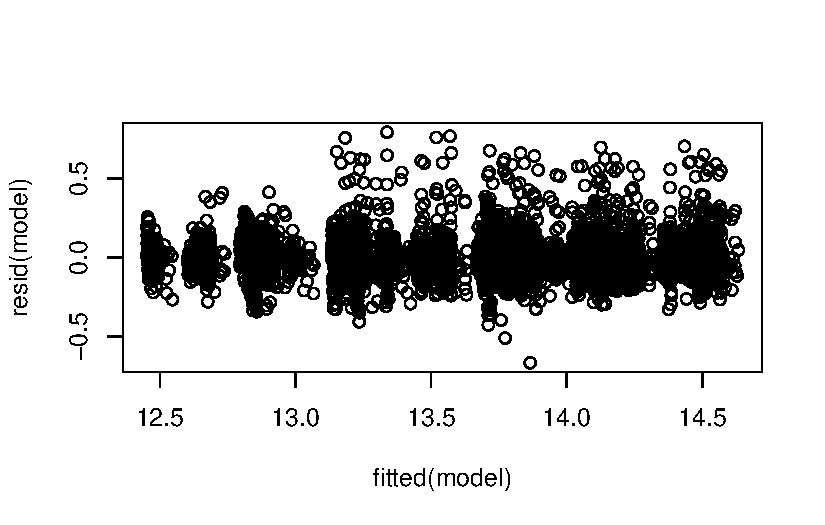
\includegraphics{678final_files/figure-pdf/unnamed-chunk-14-1.pdf}

From this plot,we can see temperatures from 25 to 75 of the country tend
to have much more numbers of higher weekly sales.

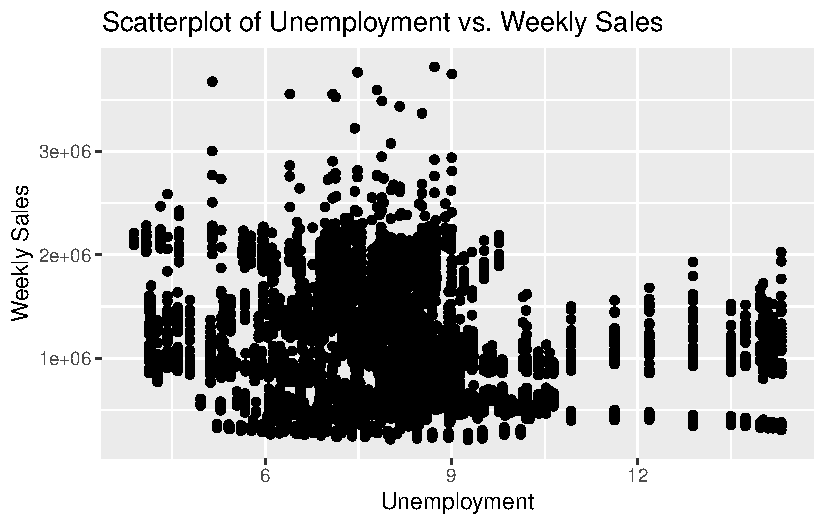
\includegraphics{678final_files/figure-pdf/unnamed-chunk-15-1.pdf}

From this plot, we can hardly see if there exist relationships between
fuel price and weekly sales.

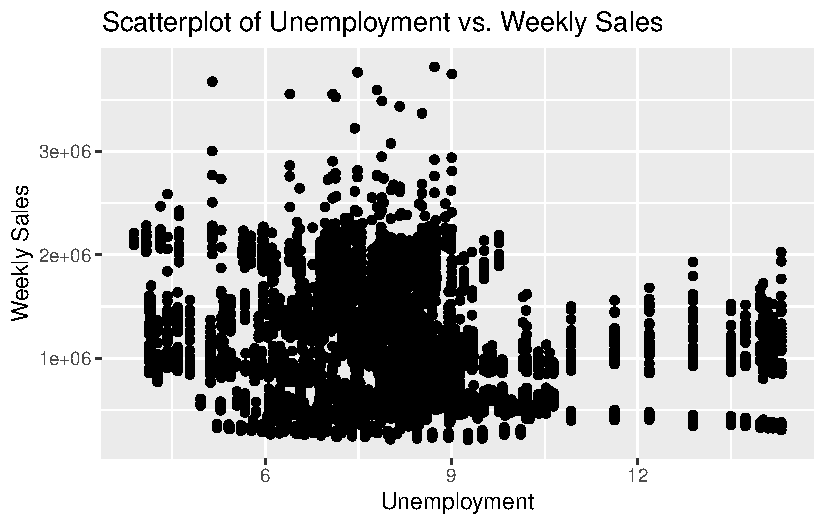
\includegraphics{678final_files/figure-pdf/unnamed-chunk-16-1.pdf}

From this plot,we can see the less of proportions of unemployment tends
to have higher weekly sales.



\end{document}
